% 
% Annual Cognitive Science Conference
% Sample LaTeX Paper -- Proceedings Format
% 

% Original : Ashwin Ram (ashwin@cc.gatech.edu)       04/01/1994
% Modified : Johanna Moore (jmoore@cs.pitt.edu)      03/17/1995
% Modified : David Noelle (noelle@ucsd.edu)          03/15/1996
% Modified : Pat Langley (langley@cs.stanford.edu)   01/26/1997
% Latex2e corrections by Ramin Charles Nakisa        01/28/1997 
% Modified : Tina Eliassi-Rad (eliassi@cs.wisc.edu)  01/31/1998
% Modified : Trisha Yannuzzi (trisha@ircs.upenn.edu) 12/28/1999 (in process)
% Modified : Mary Ellen Foster (M.E.Foster@ed.ac.uk) 12/11/2000
% Modified : Ken Forbus                              01/23/2004
% Modified : Eli M. Silk (esilk@pitt.edu)            05/24/2005
% Modified : Niels Taatgen (taatgen@cmu.edu)         10/24/2006
% Modified : David Noelle (dnoelle@ucmerced.edu)     11/19/2014

%% Change "letterpaper" in the following line to "a4paper" if you must.

\documentclass[10pt,letterpaper]{article}

\usepackage{cogsci}
\usepackage{pslatex}
\usepackage{apacite}

% our packages
% ---------------------------------------------------------
% \usepackage{hyperref}       % hyperlinks
% \usepackage{url}            % simple URL typesetting
\usepackage{subcaption}
\usepackage{amsmath,amsfonts,amsthm,amssymb,amsopn,bm}
\newcommand{\vct}[1]{\boldsymbol{#1}} % vector
\newcommand{\mat}[1]{\boldsymbol{#1}} % matrix

\usepackage{graphicx}
\graphicspath{{../graphs/}}
% ----------------------------------------------------------


\title{Selecting Between Competing Computational Models of the Stroop Task \\ On the Bases of Effective Connectivity}
 
\author{{\large \bf Micah Ketola (ketolm@uw.edu)} \\
  Department of Psychology, Campus Box 351525, \\
  Seattle, WA 98195 USA
  \AND {\large \bf Linxing Preston Jiang (prestonj@cs.washington.edu)} \\
  Paul G. Allen School of Computer Science and Engineering\\
  Seattle, WA 98195 USA 
  \AND {\large \bf Andrea Stocco (stocco@uw.edu)} \\
  Department of Psychology and Institute for Learning and Brain Sciences (I-LABS), Campus Box 351525, \\
  Seattle, WA 98195 USA}


\begin{document}

\maketitle


\begin{abstract}
\textbf{TODO} \\
Recent advances have made it possible to generate fMRI predictions for cognitive architectures, such as ACT-R, thus expanding on the possible data to be explained and making it possible to distinguish models between alternative models that make otherwise identical behavioral predictions. However, for tasks associated with relatively brief response times, fMRI predictions are often not sufficient to provide adequate identifiability. Here, we outlined a method based on effective connectivity, which significantly augments the amount of information that can be extracted from fMRi data to distinguish between model. We show the application of this method in the case of two competing ACT-R models of the Stroop task, which made identical behavioral and fMRI prediction. We show that patterns of connectivity favor on model over the other. Furthermore, we show that the same data suggests directions in which both models should be revised.

\textbf{Keywords:} 
ACT-R, Dynamic Causal Modeling, Cognitive Science
\end{abstract}


\section{Introduction}

Adaptive Control of Thought—Rational (ACT-R) \cite{Anderson2004} is a cognitive architecture which defines the basic units of human cognition processes. In most studies \cite{Anderson2004, Anderson2008, Stocco2018, Borst2017}, the focus has been put on the following modules of the architecture: visual, imaginal, goal, retrieval, manual, and procedural. The visual module is the input (e.g., perceiving visual stimuli), the manual module is the output (e.g., pressing a button for an answer), the imaginal module handles the processing of intermediate information (e.g. the middle steps to remember for solving $x$ from $\frac{2x - 5}{10} = 3$), the retrieval module contains declarative memory (e.g., common facts: the sky is blue), and the goal module controls the state of problem solving (e.g., different conditions in a task). ACT-R is a unified theory of neuroscientist-made assumptions of how these modules integrate and make up human cognition in various tasks. 

Traditionally, hemodynamic response functions (HRFs) are convolved with the event matrix (i.e., information processing of each module) derived from ACT-R to simulate fMRI data for various tasks \cite{Anderson2004,Lindquist2009}. A common choice of HRF, the double gamma function, is define as 
\[f(t, \alpha, \beta) = \frac{t^{\alpha - 1}e^{-\beta t}}{\Gamma(\alpha)}\]
where $t$ is time, $\alpha$ and $\beta$ define the scale and shape of the function, respectively, and $\Gamma(x) = (x - 1)!$ for $x \in \mathbf{R}$ \cite{Poldrack, Cignetti2016}. Then the simulated data is visually compared to the real fMRI data to check for similarities, or simple metrics such as mean square error are applied \cite{Anderson2004, Borst2017}. More rigorous analysis without the assumption of brain activations being HRF-shaped could be useful to verify ACT-R in a bottom-up approach. In this project, both brain connectivity analysis and mixture models are proposed to discover meaningful structures directly from the data with few assumptions. Specifically, covariance estimation and dynamic causal modeling were used to study brain region connectivity, and Gaussian Mixture Models were used to estimate the distributions of individual brain activation in each module.

\subsection{Experimental Task}
Real fMRI data were collected by Verstynen et al. \cite{Verstynen2014} and made publicly available on OpenNeuro at  \url{https://openneuro.org/datasets/ds000164/versions/00001}. The data was collected while the subjects performed the Stroop task \cite{Stroop1935} during which the subjects were asked to select the box whose color matched that of the text, however, the color of the text itself may (congruent trials) or may not (incongruent trials) match its semantic meaning. If, for example, the word "red" is shown on the screen painted in blue, then the subject is supposed to select the blue box instead of the red box.

\section{ACT-R Models}
This is where I'm going to put information about my models for now. 

\documentclass{article}
\usepackage{graphicx}
\begin{figure}[ht]
\centering
  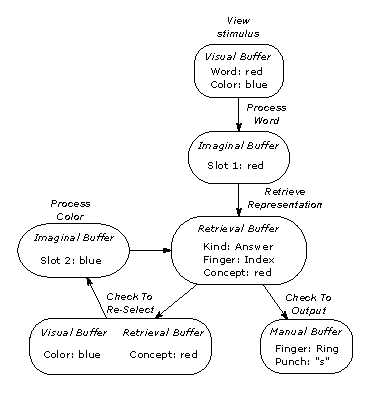
\includegraphics[width=\linewidth]{meaning_color_model.eps}
  \caption{This is my first model}
\end{figure}%

\documentclass{article}
\usepackage{graphicx}
\begin{figure}[ht]
\centering
  
\includegraphics[width=\linewidth]{overall_model.eps}
  \caption{This is my second model}
\end{figure}%


\section{Data and Modeling}

The Talairach coordinates used for each module in the brain followed the convention used by \cite{Anderson2008, Borst2017}. The algorithms described in \cite{Lacadie2008} were used to convert Talairach coordinates to Montreal Neurological Imaging Institute (MNI) coordinates (see Appendix D). The region of interest (ROI) mask files were created through FSL \cite{Woolrich2009} of size 16 mm (125 voxels in total) then used to extract fMRI data from each ROI. The real fMRI data were head-motion corrected and smoothed by a 8-mm Gaussian kernel using SPM \cite{Penny2006}. Principle component analysis was then applied on the extracted fMRI data in each ROI. The largest principle component was used to project the original data to the new space with more than 75\% of the variance explained in each module.

\subsection{Brain Connectivity Analysis}
The second type of analysis we conducted was connectivity analysis. Two types of connectivity analysis were done: (1) functional connectivity \cite{Rogers2007} which performed a covariance estimation of each brain regions with shrinkage \cite{Ledoit2004}, averaged across subjects; (2) effective connectivity through dynamic causal modeling (DCM) \cite{Friston2003, Stocco2018} which modeled the difference in brain activations through a dynamical system of other brain regions and event vectors. Specifically, DCM is expressed as a bilinear state equation
\[\dot{\vct{y}} = \mat{A}\vct{y} + \sum_{i}x_i\mat{B}(i)\vct{y} + \mat{C}\vct{x}\]
where $\mat{A}$ defines intrinsic connectivity between different regions (fixed connectivity), $\mat{C}$ defines effects by task inputs, and $\mat{B}$ defines the modular effects that task conditions have on the connectivity between regions (modulation of connectivity). The overall ``effect'' of one module
to another was then approximated by the element-wise product of $\mat{A}$ and $\mat{B}$, namely
\[\text{effective connectivity} = \mat{A} \odot \mat{B}\]
Since each trial the Stroop task is generally performed within one second, it is expected that the three information processing modules: imaginal, goal, and retrieval should have strong correlations since their activation could only be captured in one image scan given our sampling rate $TR = 1.5$ seconds. Furthermore, if the imaginal module is for intermediate information processing as ACT-R suggests, an increasing connectivity effect from imaginal module to goal module ("problem state") is expected in order to process the unmatching color and text semantics in incongruent trials.

\section{Result}

Figure~\ref{fig:conn} shows the connectivity analysis results between modules. Figure~\ref{fig:conn} (a) shows the functional connectivity between retrieval and imaginal is high as expected, while that between imaginal and goal is not as high. (b) and (c) show the results of DCM in both congruent and incongruent trials averaged across subjects through Bayesian parameter averaging \cite{Kasess2010} (see Appendix C), and (d) shows the difference in the effective connectivity in different tasks (incongruent - congruent). Circled parts in (d) confirm the effect we expect from ACT-R: in incongruent trials, there is a significant increase between imaginal and goal modules to account for the unmatching color and semantic condition. More importantly, their effect on the output (i.e., the manual module) also changes drastically. Compared to congruent trials, there is a significant decrease effect from goal to manual and a significant increase effect from imaginal to manual, suggesting that information about the final decision is delivered by imaginal rathar than goal in incongruent trials. Again, this supports ACT-R's assumption that little imaginal involvement is needed in congruent trials. 



\section{Formalities, Footnotes, and Floats}

Use standard APA citation format. Citations within the text should
include the author's last name and year. If the authors' names are
included in the sentence, place only the year in parentheses, as in
\citeA{NewellSimon1972a}, but otherwise place the entire reference in
parentheses with the authors and year separated by a comma
\cite{NewellSimon1972a}. List multiple references alphabetically and
separate them by semicolons
\cite{ChalnickBillman1988a,NewellSimon1972a}. Use the
``et~al.'' construction only after listing all the authors to a
publication in an earlier reference and for citations with four or
more authors.


\subsection{Footnotes}

Indicate footnotes with a number\footnote{Sample of the first
footnote.} in the text. Place the footnotes in 9~point type at the
bottom of the column on which they appear. Precede the footnote block
with a horizontal rule.\footnote{Sample of the second footnote.}


\subsection{Tables}

Number tables consecutively. Place the table number and title (in
10~point) above the table with one line space above the caption and
one line space below it, as in Table~\ref{sample-table}. You may float
tables to the top or bottom of a column, or set wide tables across
both columns.

\begin{table}[!ht]
\begin{center} 
\caption{Sample table title.} 
\label{sample-table} 
\vskip 0.12in
\begin{tabular}{ll} 
\hline
Error type    &  Example \\
\hline
Take smaller        &   63 - 44 = 21 \\
Always borrow~~~~   &   96 - 42 = 34 \\
0 - N = N           &   70 - 47 = 37 \\
0 - N = 0           &   70 - 47 = 30 \\
\hline
\end{tabular} 
\end{center} 
\end{table}


\subsection{Figures}

All artwork must be very dark for purposes of reproduction and should
not be hand drawn. Number figures sequentially, placing the figure
number and caption, in 10~point, after the figure with one line space
above the caption and one line space below it, as in
Figure~\ref{sample-figure}. If necessary, leave extra white space at
the bottom of the page to avoid splitting the figure and figure
caption. You may float figures to the top or bottom of a column, or
set wide figures across both columns.

\begin{figure}[ht]
\centering
\begin{subfigure}{.5\textwidth}
  \centering
  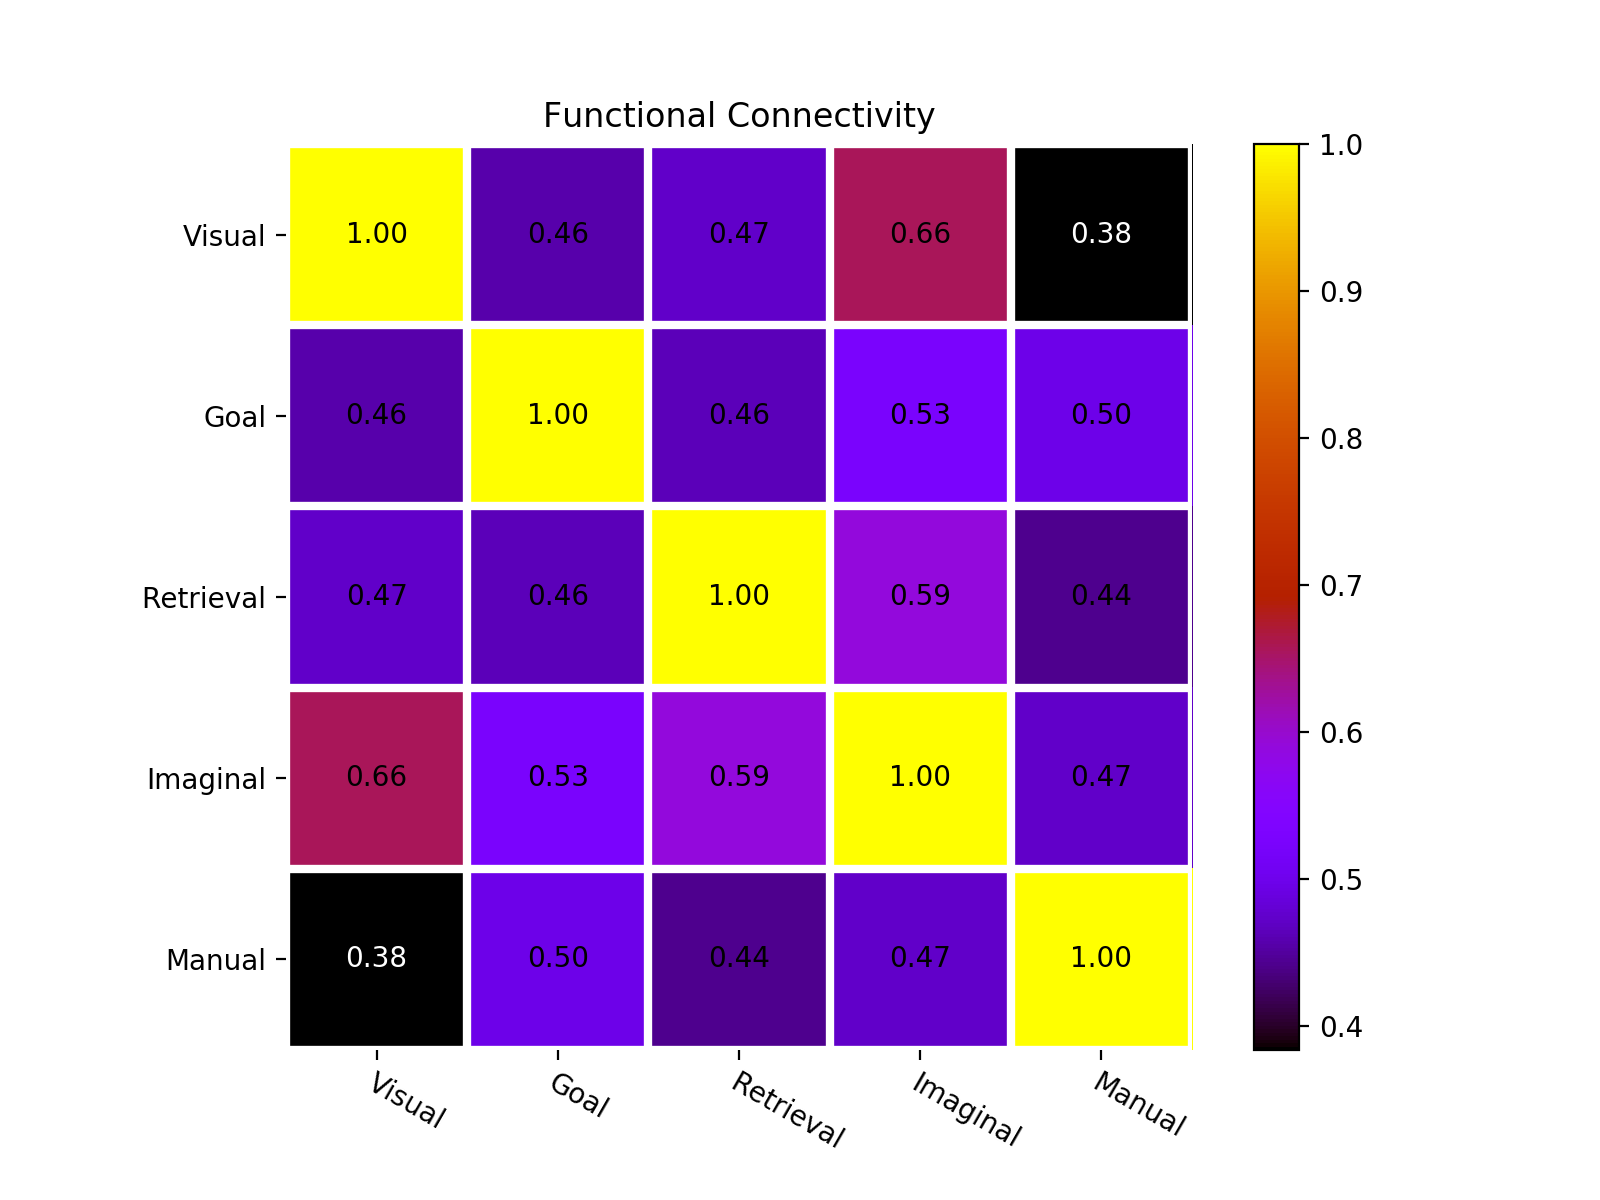
\includegraphics[width=\linewidth]{func_conn.png}
  \caption{}
\end{subfigure}%
\begin{subfigure}{.5\textwidth}
  \centering
  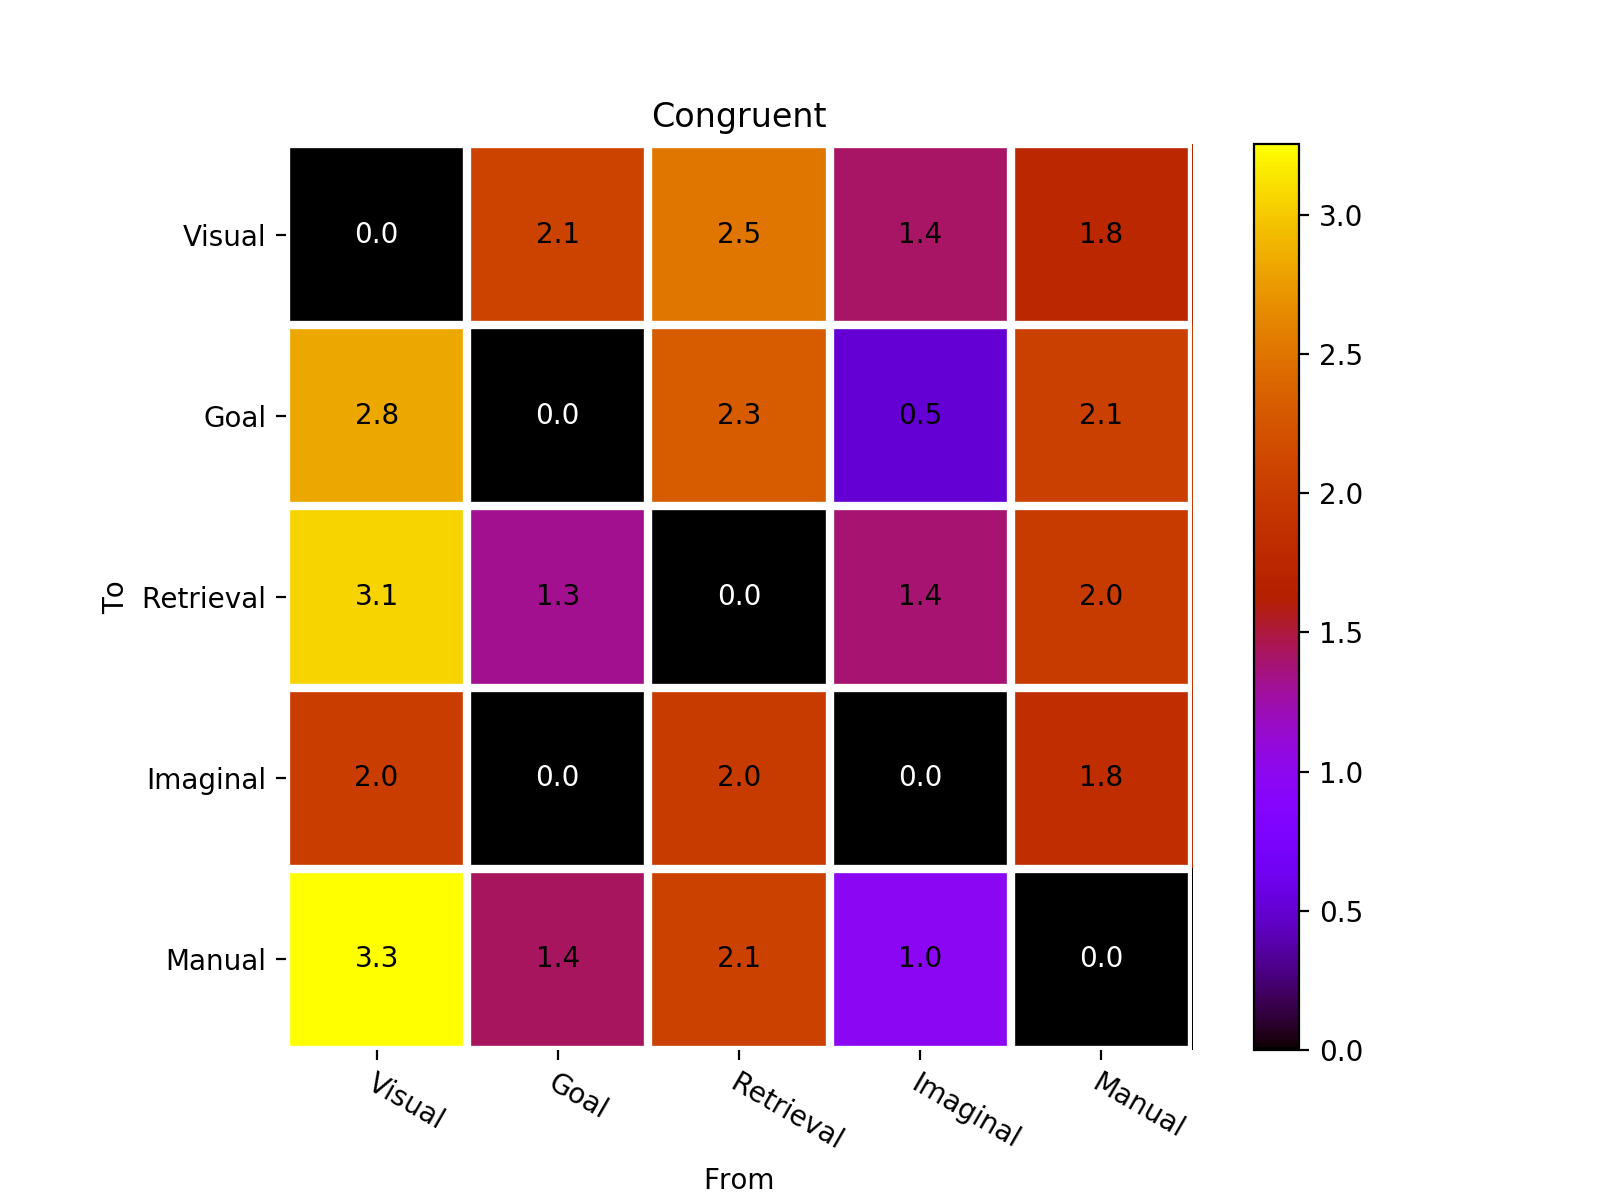
\includegraphics[width=\linewidth]{Congruent_effect_conn.png}
  \caption{}
\end{subfigure}
\begin{subfigure}{.5\textwidth}
  \centering
  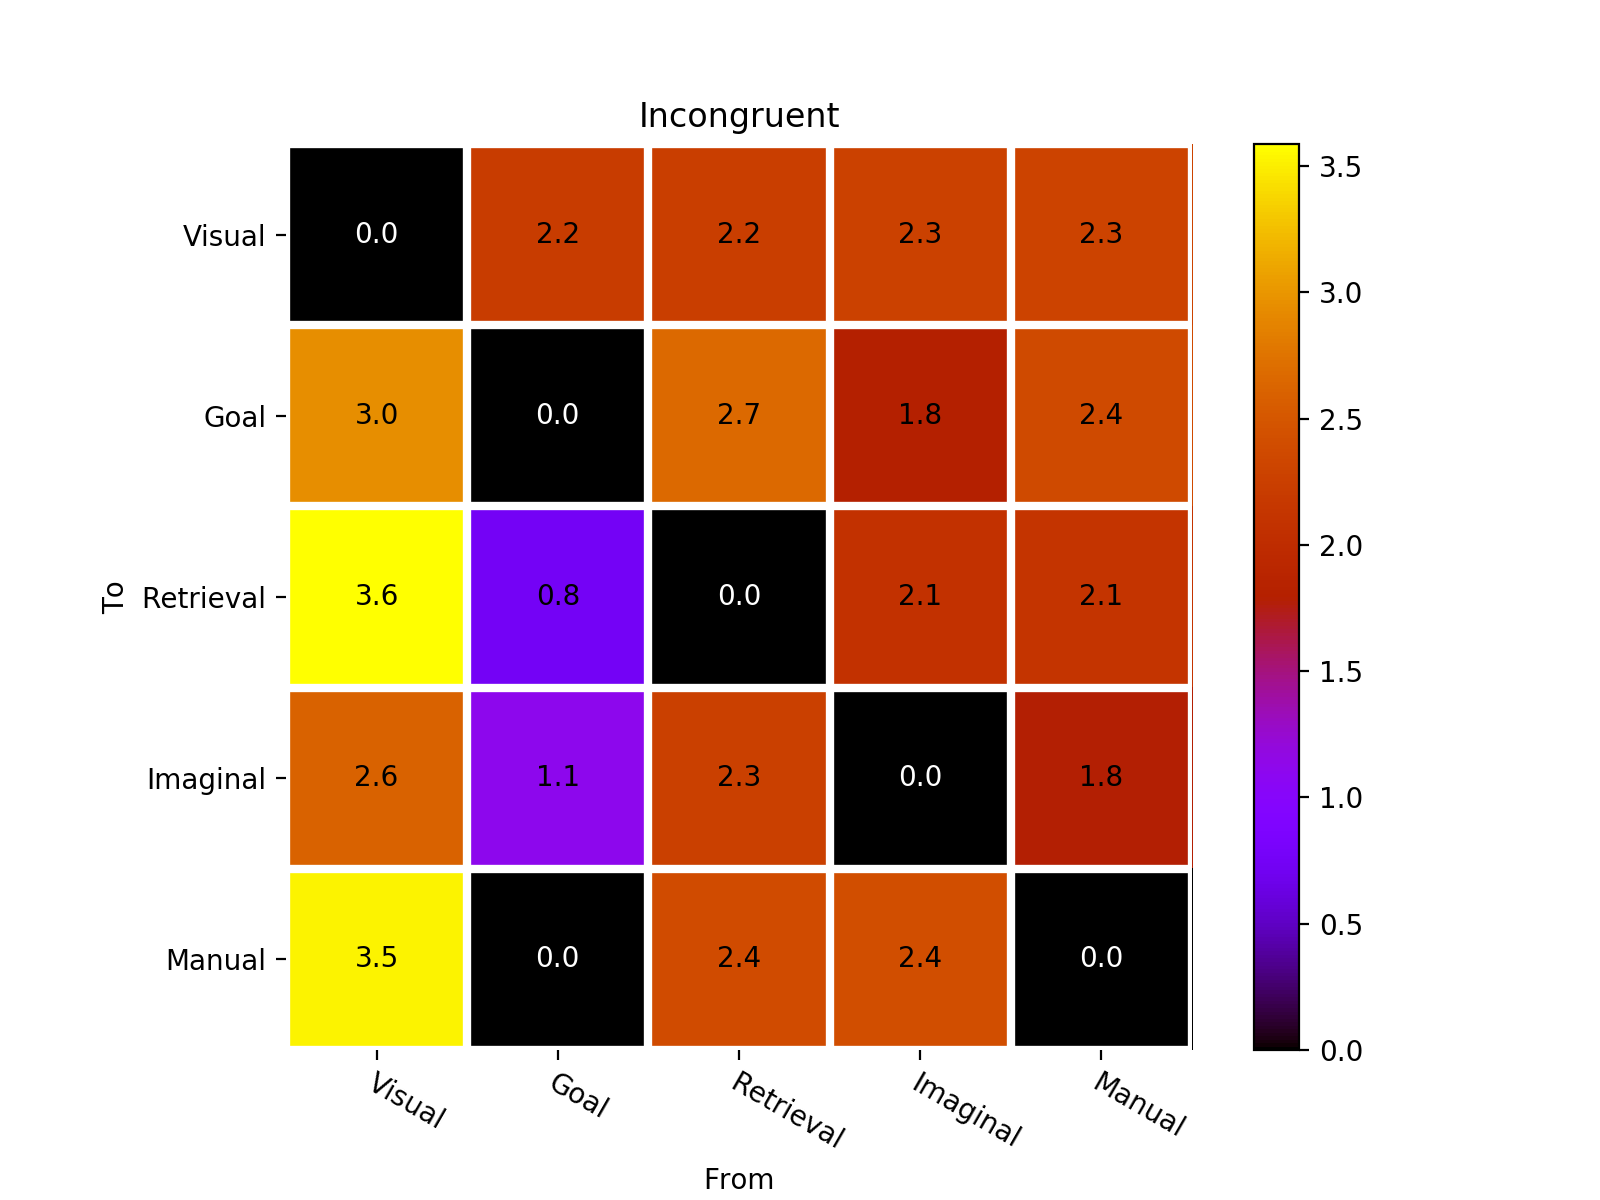
\includegraphics[width=\linewidth]{Incongruent_effect_conn.png}
  \caption{}
\end{subfigure}%
\begin{subfigure}{.5\textwidth}
  \centering
  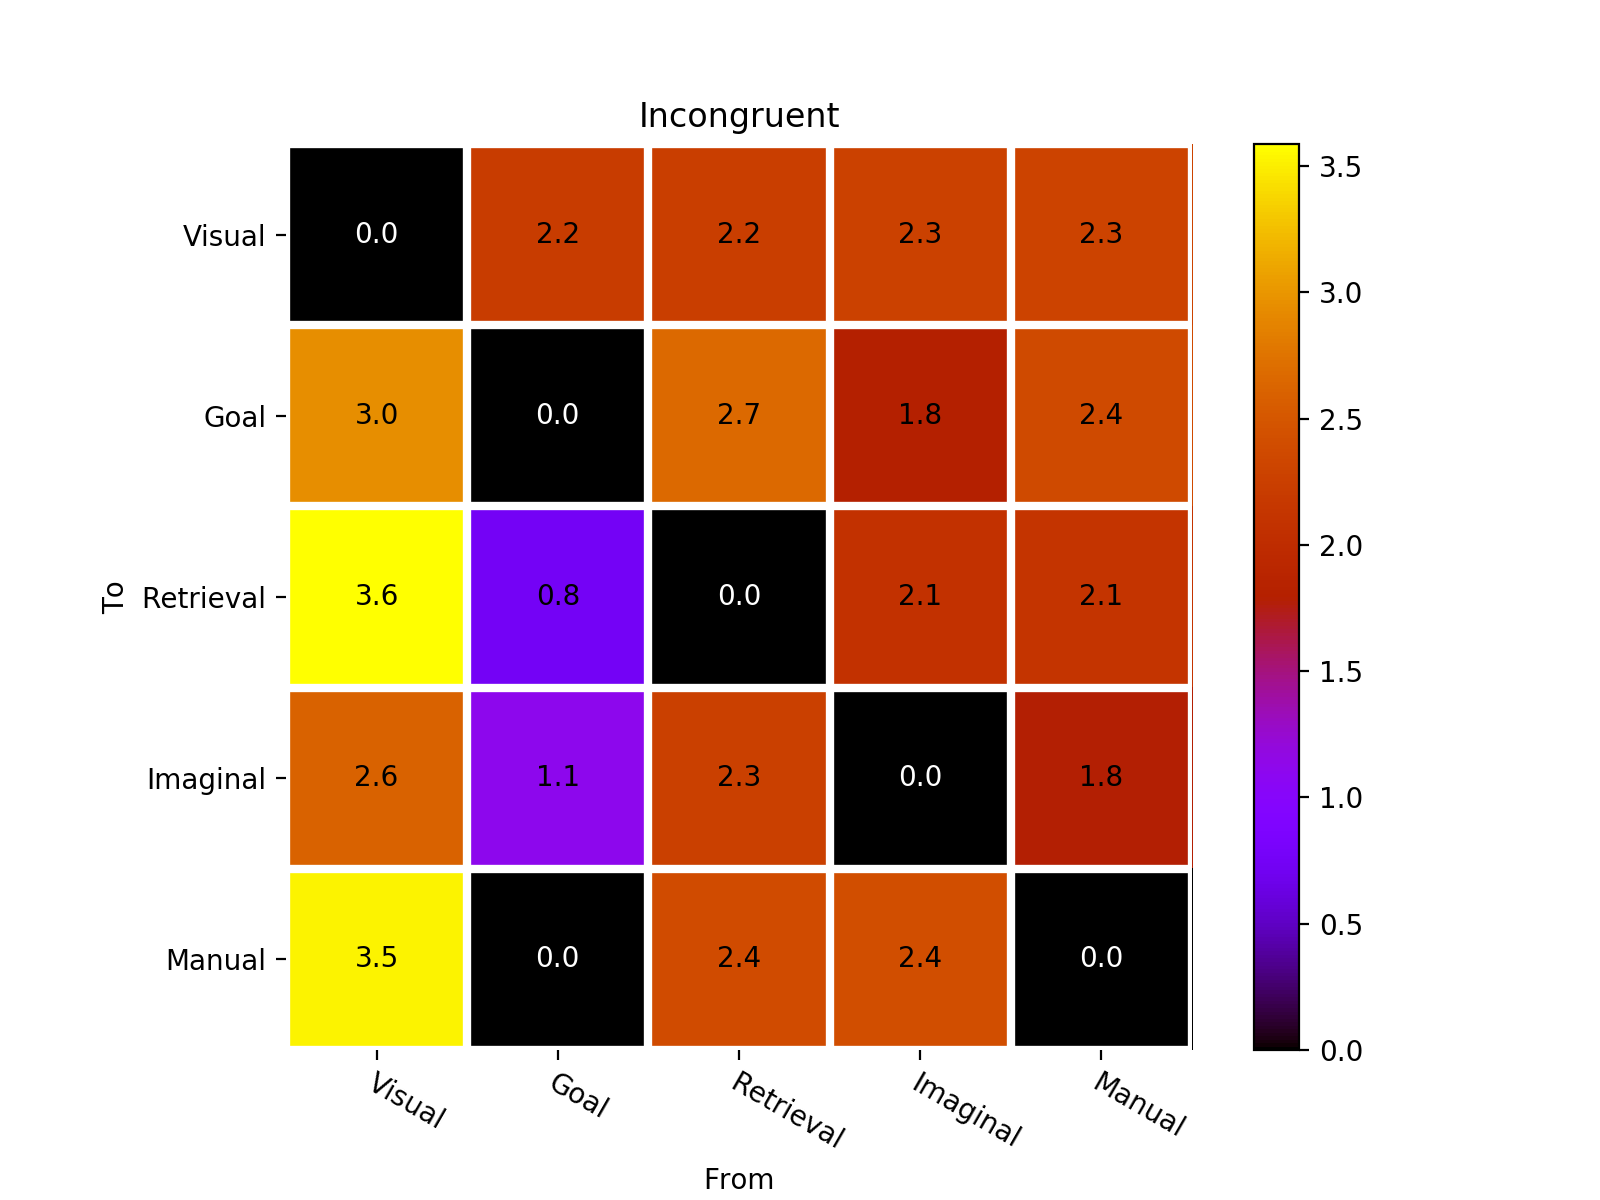
\includegraphics[width=\linewidth]{Incongruent_effect_conn.png}
  \caption{}
\end{subfigure}
\caption{Brain region connectivity results: (a) Functional connectivity analysis shows strong brain signal activation between imaginal and retrieval, but not imaginal and goal; (b) Effective connectivity in congruent trials: similar strong effects between retrieval and imaginal are shown (data is zero-min) ; (c) Effective connectivity in incongruent trials: increasing connectivity between imaginal and goal are shown (data is zero-min); (d) Difference of effective connectivity in different tasks (incongruent - congruent): circled regions show brain connectivity dynamics in different tasks.}
\label{fig:conn}
\end{figure}


\begin{figure}[ht]
\begin{center}
\fbox{CoGNiTiVe ScIeNcE}
\end{center}
\caption{This is a figure.} 
\label{sample-figure}
\end{figure}


\section{Acknowledgments}

Place acknowledgments (including funding information) in a section at
the end of the paper.


\section{References Instructions}

Follow the APA Publication Manual for citation format, both within the
text and in the reference list, with the following exceptions: (a) do
not cite the page numbers of any book, including chapters in edited
volumes; (b) use the same format for unpublished references as for
published ones. Alphabetize references by the surnames of the authors,
with single author entries preceding multiple author entries. Order
references by the same authors by the year of publication, with the
earliest first.

Use a first level section heading, ``{\bf References}'', as shown
below. Use a hanging indent style, with the first line of the
reference flush against the left margin and subsequent lines indented
by 1/8~inch. Below are example references for a conference paper, book
chapter, journal article, dissertation, book, technical report, and
edited volume, respectively.

\nocite{ChalnickBillman1988a}
\nocite{Feigenbaum1963a}
\nocite{Hill1983a}
\nocite{OhlssonLangley1985a}
% \nocite{Lewis1978a}
\nocite{Matlock2001}
\nocite{NewellSimon1972a}
\nocite{ShragerLangley1990a}


\bibliographystyle{apacite}

\setlength{\bibleftmargin}{.125in}
\setlength{\bibindent}{-\bibleftmargin}

\bibliography{ref}


\end{document}
